\documentclass{crocs-slide}
%\documentclass[bw]{crocs-slide}
%\documentclass[nologo]{crocs-slide}
%\documentclass[bw, nologo]{crocs-slide}

\usepackage[english]{babel}

\title{Edu-hoc}
\subtitle{https://github.com/crocs-muni/Edu-hoc}
\author[L. Němec]{%
\makebox[0.5\textwidth][l]{\textbf{Lukáš Němec}}\\%
\vskip 1em
\makebox[0.5\textwidth][l]{lukas.nemec@mail.muni.cz}\\%
%\vskip 1em
%\makebox[0.5\textwidth][l]{Tommy Atkins}%
}
\date{\today}
\begin{document}

  \maketitle


  \begin{frame}
    \frametitle{Motivation}

    \textbf{Wireless sensor networks:}
    \vskip 2em
    Distributed autonomous devices with sensors
    \vskip 1em
    Limited by CPU, memory, radio range, energy \dots
    \vskip 1em
    Multi-hop mesh network with $10^2 ~ - ~ 10^6$ nodes
    \vskip 1em
    Specialized OS (TinyOS, Contiki OS)

  \end{frame}




  \begin{frame}
    \frametitle{Motivation II.}
    \framesubtitle{WSN problem}
    Hop by Hop communication
    \vskip 1em
    Specialized OS with non usual language (e.g. NesC)
    \vskip 1em
    common tasks are not trivial
    \vskip 1em
    \begin{itemize}
      \item Routing
      \item Security
      \item Intrusion detection
      \item Key exchange
      \item \dots
    \end{itemize}

  \end{frame}

  \begin{frame}
    \frametitle{Edu-hoc Solution}
    \begin{columns}
      \column{0.7\textwidth}
      \begin{itemize}
        \item Arduino based network
        \vskip 1em
        \item simple C code
        \vskip 1em
        \item set of exercises (scenarios)
        \vskip 1em
        \item solve scenarios as attacker
        \vskip 1em
        \item Fix code to prevent such attack
      \end{itemize}
      \column{0.3\textwidth}
      \begin{figure}
        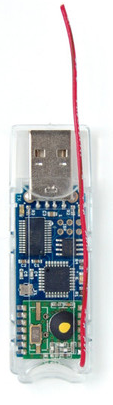
\includegraphics[scale=0.4]{jeeLink.png}
        \caption{JeeLink node}
      \end{figure}
    \end{columns}

  \end{frame}
  \begin{frame}
    \frametitle{Exercises}

    5 scenarios
    \vskip 1em
    Each with different objective
    \vskip 1em
    Evaluation as percentage of messages
    \begin{itemize}
      \item captured
      \vskip 1em
      \item delivered
      \vskip 1em
      \item modified
    \end{itemize}

  \end{frame}

  \begin{frame}
    \frametitle{Exercises}
    \textbf{1. Eavesdropping}
    \vskip 1em
    Unsecured network
    \vskip 1em
    Global broadcast from each node
    \vskip 1em
    Capture as many messages as possible
    \vskip 1em


  \end{frame}

  \begin{frame}
    \frametitle{Exercises}
    \framesubtitle{Routing attacks}
    \textbf{2. Black hole}
    \vskip 1em
    Network with dynamic routing
    \vskip 1em
    Initial phase of route establishment
    \vskip 1em
    Prevent as many packets from reaching BS
    \vskip 2em
    \textbf{3. Sink hole}
    \vskip 1em
    Deliver as many modified packets as possible
    \vskip 1em
    Capture, modify and send back

  \end{frame}

  \begin{frame}
    \frametitle{Exercises}
    \textbf{4. Jamming}
    \vskip 1em
    Secured network with fixed routing
    \vskip 1em
    Prevent as many packets from reaching BS
    \vskip 1em
    No way to modify routes etc.
    \vskip 2em
    \textbf{5. Relay attack}
    \vskip 1em
    Network with dynamic routing
    \vskip 1em
    Initial phase of route establishment
    \vskip 1em
    Modify the routes to be longer or shorter

  \end{frame}

  \begin{frame}
    \frametitle{Infrastructure behind I.}
    \framesubtitle{Network}
    Network of  approximately 20 nodes
    \begin{figure}[!ht]

      \centering
    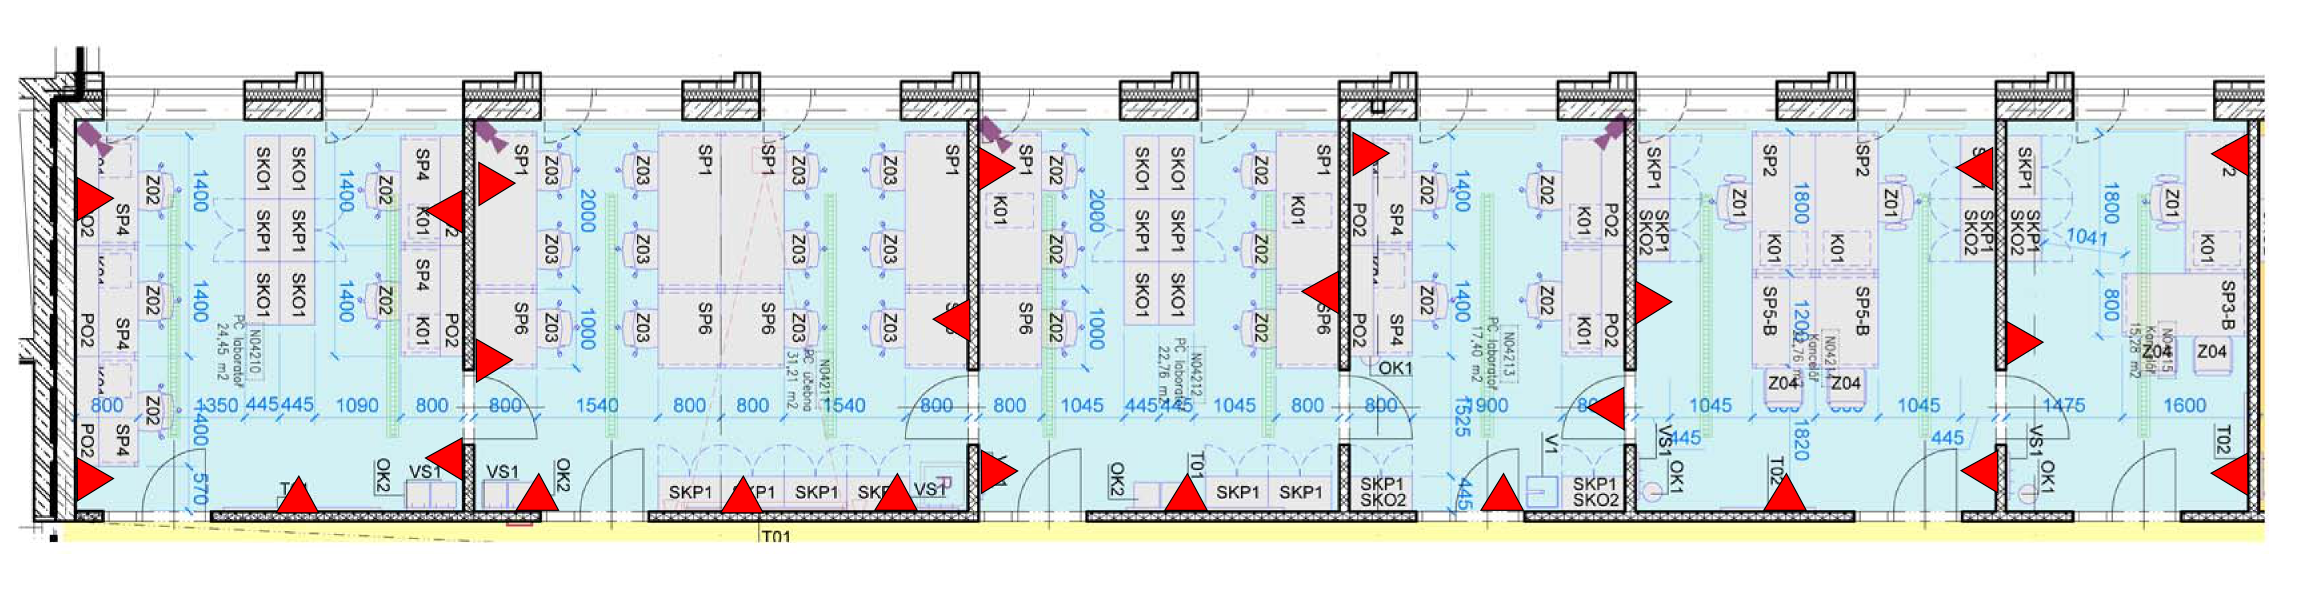
\includegraphics[width=\textwidth]{net.png}
    \caption{Network placement}
\end{figure}


  \end{frame}

  \begin{frame}
    \frametitle{Infrastructure behind II.}
    \framesubtitle{Network management}
    Network of  approximately 20 nodes
    \vskip 1em
    Impossible to be managed one by one
    \pause
    \vskip 1em
    Mass configuration for nodes
    \vskip 1em
    Mass communication (IN and OUT) with nodes

  \end{frame}

  \begin{frame}
    \frametitle{Infrastructure behind III.}
    \framesubtitle{Scenarios evaluation}
    Unique message generator
    \vskip 1em
    Unique identifier for each participant
    \vskip 1em
    BS (computer with dedicated node) with capability to:
    \vskip 1em
    \begin{itemize}
      \item show current network state on web page
      \item start scenario
      \item collect scenario results from nodes
      \item evaluate results and show them on web page
      \item assign results per participant (if applicable)
    \end{itemize}

  \end{frame}

  \begin{frame}
    \frametitle{Current usage}
    \framesubtitle{PA197}
    3 seminars dedicated to WSN hands on work
    \vskip 1em
    First and third scenarios used as homework
    \vskip 1em
    36 students
    \vskip 1em
    Submitted files evaluated manually


  \end{frame}

  \begin{frame}
    \frametitle{Project state}
    \textbf{Implemented:}
    \begin{itemize}
      \item Tools for network management
      \item 5 scenarios with solutions
      \item Example applications (Sniffer, \dots)
      \item Evaluation scripts (used manually or automatically)
      \item Web interface with network status
      \item Scenario deployment scripts (automated runs)
    \end{itemize}
    \textbf{Remaining:}
    \begin{itemize}
      \item Automated evaluation of submitted files via web interface
    \end{itemize}

  \end{frame}

  \begin{frame}
    \frametitle{Edu-hoc}
    \framesubtitle{https://github.com/crocs-muni/Edu-hoc}

    \begin{LARGE}
      \begin{center}
        Thank you for your attention

        \vskip 3em

        Questions?
      \end{center}
    \end{LARGE}

  \end{frame}

\end{document}
